% !TeX root = ../tfg.tex
% !TeX encoding = utf8
%
%*******************************************************
% Capítulo 11. STOOD-X
%*******************************************************

\chapter{STOOD-X}\label{cap:stoodx}

% Descripción del método en la \cref{sec:metodo-stoodx}. Fuentes: results_ood/faseB_paper_2026-10-20,
% results_ood/stoodx_validacion y faseC. Selección de K: results_ood/stoodx_seleccion_k; evaluación con
% K = 144: results_ood/faseB_paper_K144 y faseC_K144. Todo con el Swin-S.
\pendiente{introducción del capítulo}

\section{Implementación}\label{sec:stoodx-implementacion}

El método se ha implementado siguiendo la descripción del artículo~\cite{sevillano2026}. Se realiza un único test por imagen entre las $K$ distancias de $x$ y las $K^2$ distancias de sus vecinos mediante \texttt{scipy.stats.mannwhitneyu} (Virtanen et al.~\cite{virtanen2020}).

% Puntos que debería cubrir (tono neutro y descriptivo: el tutor Iván Sevillano es primer autor
% del método):
% - La implementación pública difiere del texto del artículo: la referencia de cada test es la
%   i-ésima imagen de entrenamiento de la clase predicha y no los vecinos de los vecinos, y el test
%   es de Wilcoxon pareado (RESUMEN_STOODX.md, «Problemas encontrados», punto 1).
% - Por ello se reimplementó según el texto del artículo; interpretación pendiente de confirmar
%   con los autores.
% - Coste: ~1 ms/imagen en GPU + ~11-13 ms/imagen en CPU; ~25 min por configuración para las
%   122.208 imágenes. Con K = 144: 0,03-0,05 ms/imagen en GPU + 0,82-0,88 ms/imagen en CPU
%   (slurm-stoodx-paper-192888.out, 8 procesos, Quadro RTX 8000).
\pendiente{diferencias entre la implementación pública y la descripción del artículo, y motivo de la reimplementación}
\revisar{tono}

\section{Configuración}\label{sec:stoodx-configuracion}

Se emplean la distancia coseno, $K = 500$ (el valor seleccionado en el artículo), el conjunto de entrenamiento ID de la clase predicha como referencia y dos configuraciones de características: el 100\,\% y el 87,5\,\% más presente. Dado que el criterio de relevancia del artículo se basa en CRP (\cref{sec:crp}), que no es directamente aplicable a un Swin Transformer, la selección del 87,5\,\% se realiza mediante la presencia de cada característica (suma de sus valores absolutos en la clase), criterio utilizado en la implementación pública. Ningún hiperparámetro se ha ajustado con datos OOD.
\revisar{tono}

% Además, una variante exploratoria K_c = \min(500, \lfloor n_c/2 \rfloor), propuesta tras ver la
% validación con datos OOD (\cref{sec:stoodx-k}); 87,5 % = 672 de 768 características.

\subsection{Selección de \texorpdfstring{$K$}{K}}\label{sec:stoodx-seleccion-k}

El valor $K = 500$ se fijó en el artículo para sus propios conjuntos de datos, y en este problema varias clases tienen menos de 500 imágenes de entrenamiento o pocas más (\cref{sec:stoodx-k}). Elegir $K$ con los resultados del test ID o de los conjuntos OOD daría una estimación optimista del rendimiento (\emph{data snooping}), por lo que se ha seleccionado mediante una validación \emph{leave-one-class-out} que solo usa datos ID. Para cada una de las 14 clases ID $h$:
\begin{itemize}
  \item se eliminan de la referencia de entrenamiento las imágenes con etiqueta $h$;
  \item se anula el logit de $h$, de modo que el modelo predice entre las 13 clases restantes;
  \item las imágenes de validación de la clase $h$ hacen de pseudo-OOD frente al resto de la validación ID.
\end{itemize}
Se prueban los mismos valores que en el artículo, $K \in \{9, 18, 36, 72, 144, 288, 500\}$, con el 100\,\% de las características y la puntuación $-z$. La regla de decisión se fijó en el código antes de ver los resultados: se elige el $K$ con mayor \AUROC medio sobre las 14 clases y, en caso de empate con tres decimales, el más pequeño. No se utiliza ningún dato del test ID ni de los conjuntos OOD.

% Generado por scripts/generar_tablas.py a partir de results_ood/stoodx_seleccion_k/seleccion_k_loco.csv y seleccion_k_loco_por_clase.csv. No editar a mano.
\begin{table}[tbp]
\centering
\footnotesize
\caption{Selección de $K$ de \stoodx (100\,\% de las características, puntuación $-z$) por validación \emph{leave-one-class-out} en la validación ID: cada una de las 14 clases ID hace por turno de pseudo-OOD frente al resto de la validación, sin sus imágenes en la referencia de entrenamiento y con su logit anulado. \AUROC (más alto es mejor) y \FPRn{95} (más bajo es mejor) medios sobre las 14 clases, y número de clases retenidas en las que cada $K$ obtiene el mayor \AUROC. En negrita, el $K$ elegido. No se usa ningún dato de test ni OOD.}
\label{tab:stoodx-seleccion-k}
\begin{tabular}{cccc}
\toprule
$K$ & \AUROC medio $\uparrow$ & \FPRn{95} medio $\downarrow$ & Clases en que es el mejor \\
\midrule
9 & 0{,}844 & 0{,}418 & 0 \\
18 & 0{,}898 & 0{,}310 & 0 \\
36 & 0{,}929 & 0{,}235 & 1 \\
72 & 0{,}949 & 0{,}178 & 0 \\
\textbf{144} & \textbf{0{,}961} & 0{,}145 & 10 \\
288 & 0{,}946 & 0{,}325 & 2 \\
500 & 0{,}934 & 0{,}415 & 1 \\
\bottomrule
\end{tabular}
\end{table}


El valor elegido es $K = 144$, con un \AUROC medio de 0,961 y un \FPRn{95} medio de 0,145, frente a 0,934 y 0,415 con $K = 500$ (\cref{tab:stoodx-seleccion-k}). Es también el mejor $K$ en 10 de las 14 clases retenidas; en las otras cuatro gana $K = 288$ (\clase{Estroma} y \clase{Glandulas\_no\_neoplasicas}), $K = 36$ (\clase{Gleason\_4\_glomeruloide}) o $K = 500$ (\clase{Gleason\_4\_pobremente\_formadas}).

Este criterio tiene tres limitaciones. En primer lugar, supone que una clase ID retenida se comporta como un OOD real, cuando es un cambio semántico entre clases de próstata y no un cambio de centro, de tejido o de escala como los de los conjuntos OOD (\cref{sec:conjuntos-ood}). En segundo lugar, la selección y la evaluación con $K = 144$ se han hecho solo con el Swin-S: la repetición con ConvNeXt-S (\cref{ap:convnext}) y el experimento de corrupciones (\cref{sec:corrupciones}) mantienen $K = 500$, por lo que sus cifras de \stoodx no son comparables con las de $K = 144$. En tercer lugar, la calibración de los $p$-valores (\cref{sec:stoodx-calibracion}) solo se ha estudiado con $K = 500$.
\revisar{subsección redactada por el agente a petición del autor (excepción a la regla de no redactar prosa); revisar estilo y contenido}

% Cifras (results_ood/stoodx_seleccion_k/): AUROC medio por K: 0,844 / 0,898 / 0,929 / 0,949 / 0,961 /
% 0,946 / 0,934; FPR@95 medio: 0,418 / 0,310 / 0,235 / 0,178 / 0,145 / 0,325 / 0,415. La clase
% Gleason_4_glomeruloide solo tiene 43 imágenes de validación (pseudo-OOD), así que su AUROC es ruidoso.
% Log: slurm-stoodx-paper-192374.out.

\section{Puntuación}\label{sec:stoodx-puntuacion}

Como puntuación de detección se utiliza el estadístico tipificado del test de Mann-Whitney, $z$, obtenido mediante la aproximación normal del estadístico $U$ con corrección por empates y por continuidad (\cref{teo:u-normal,obs:u-empates}). Dado que $p = 1 - \Phi(z)$ es una función monótona decreciente de $z$, la puntuación $-z$ induce la misma ordenación que el $p$-valor propuesto en STOOD-X, pero evita el subdesbordamiento numérico que se produce cuando $p < 10^{-308}$. Cuando todas las distancias de $x$ superan a las de sus vecinos (separación completa), el estadístico alcanza su valor máximo y varias imágenes quedan empatadas. Con $K = 500$, esto afecta al 66\,\% de TUM + NORM pero solo al 0,6\,\% del test ID; su efecto está acotado en $\pm 0{,}003$ en AUROC, y no altera FPR@95 ni CCR@FPR5 (\cref{tab:stoodx-saturacion}).

% Generado por scripts/generar_tablas.py a partir de results_ood/faseB_paper_2026-10-20/empates_saturacion.csv. No editar a mano.
\begin{table}
\centering
\footnotesize
\setlength{\tabcolsep}{4pt}
\caption{Saturación de la puntuación $-z$ de \stoodx (100\,\%, $K=500$) por separación completa: proporción de imágenes con $U=n_1n_2$ y cotas de su efecto en el \AUROC (más alto es mejor), forzando el peor y el mejor orden entre las imágenes ID y OOD saturadas. \FPRn{95} y \CCRn{5} no cambian en ningún conjunto.}
\label{tab:stoodx-saturacion}
\begin{tabular*}{\linewidth}{@{\extracolsep{\fill}}lccccc}
\toprule
Conjunto & Saturadas test ID & Saturadas OOD & \AUROC & \AUROC peor caso & \AUROC mejor caso \\
\midrule
TUM+NORM & 0{,}6\,\% & 66{,}3\,\% & 0{,}953 & 0{,}951 & 0{,}955 \\
TUM & 0{,}6\,\% & 59{,}0\,\% & 0{,}931 & 0{,}929 & 0{,}933 \\
NORM & 0{,}6\,\% & 78{,}2\,\% & 0{,}990 & 0{,}987 & 0{,}992 \\
STR & 0{,}6\,\% & 52{,}0\,\% & 0{,}978 & 0{,}976 & 0{,}979 \\
LYM & 0{,}6\,\% & 32{,}1\,\% & 0{,}903 & 0{,}903 & 0{,}905 \\
MUS & 0{,}6\,\% & 44{,}1\,\% & 0{,}968 & 0{,}966 & 0{,}969 \\
PANDA & 0{,}6\,\% & 19{,}4\,\% & 0{,}895 & 0{,}895 & 0{,}896 \\
Control 128\,px & 0{,}6\,\% & 19{,}0\,\% & 0{,}894 & 0{,}893 & 0{,}895 \\
DTD & 0{,}6\,\% & 76{,}3\,\% & 0{,}991 & 0{,}987 & 0{,}992 \\
\bottomrule
\end{tabular*}
\end{table}


Con $K = 144$, la saturación no desaparece, pero no afecta a las conclusiones. Ningún $p$-valor se anula por subdesbordamiento y el \AUROC calculado con $p$ coincide con el de $-z$, pero la separación completa es más frecuente que con $K = 500$: afecta al 1,2\,\% del test ID, al 86\,\% de TUM+NORM y al 90\,\% de DTD (\cref{tab:stoodx-saturacion-k144}). Su efecto sigue acotado: \FPRn{95} y \CCRn{5} no cambian en ningún conjunto, y el \AUROC se mueve como mucho $\pm 0{,}007$ (TUM+NORM: 0,991 en [0,985; 0,996]). Incluso en el peor caso, \stoodx con $K = 144$ supera al mejor método de OpenOOD en todos los conjuntos salvo LYM. Además, como todas las clases tienen más de $K = 144$ imágenes de entrenamiento, el valor máximo de $z$ es el mismo para todas, y desaparece la diferencia de escala entre clases que había con $K = 500$ en las clases pequeñas (\cref{sec:stoodx-k}).
\revisar{párrafo redactado por el agente a petición del autor; revisar}

% Generado por scripts/generar_tablas.py a partir de results_ood/faseB_paper_K144/empates_saturacion.csv. No editar a mano.
\begin{table}
\centering
\footnotesize
\setlength{\tabcolsep}{4pt}
\caption{Saturación de la puntuación $-z$ de \stoodx (100\,\%, $K=144$) por separación completa: proporción de imágenes con $U=n_1n_2$ y cotas de su efecto en el \AUROC (más alto es mejor), forzando el peor y el mejor orden entre las imágenes ID y OOD saturadas. \FPRn{95} y \CCRn{5} no cambian en ningún conjunto.}
\label{tab:stoodx-saturacion-k144}
\begin{tabular}{lccccc}
\toprule
Conjunto & Saturadas test ID & Saturadas OOD & \AUROC & \AUROC peor caso & \AUROC mejor caso \\
\midrule
TUM+NORM & 1{,}2\,\% & 86{,}4\,\% & 0{,}991 & 0{,}985 & 0{,}996 \\
TUM & 1{,}2\,\% & 84{,}1\,\% & 0{,}990 & 0{,}985 & 0{,}995 \\
NORM & 1{,}2\,\% & 90{,}3\,\% & 0{,}992 & 0{,}986 & 0{,}998 \\
STR & 1{,}2\,\% & 69{,}8\,\% & 0{,}982 & 0{,}977 & 0{,}985 \\
LYM & 1{,}2\,\% & 64{,}9\,\% & 0{,}966 & 0{,}961 & 0{,}969 \\
MUS & 1{,}2\,\% & 62{,}8\,\% & 0{,}977 & 0{,}973 & 0{,}981 \\
PANDA & 1{,}2\,\% & 30{,}1\,\% & 0{,}939 & 0{,}938 & 0{,}942 \\
Control 128\,px & 1{,}2\,\% & 39{,}4\,\% & 0{,}935 & 0{,}932 & 0{,}936 \\
DTD & 1{,}2\,\% & 90{,}0\,\% & 0{,}993 & 0{,}986 & 0{,}997 \\
\bottomrule
\end{tabular}
\end{table}


% Cifras (faseB_paper_K144/empates_saturacion.csv, analisis_empates_stoodx.py con K = 144): saturadas
% OOD: TUM+NORM 86,4 %, TUM 84,1 %, NORM 90,3 %, STR 69,8 %, LYM 64,9 %, MUS 62,8 %, PANDA 30,1 %,
% control 39,4 %, DTD 90,0 %; test ID 1,2 % (0,6 % con K = 500). Máxima variación de AUROC: DTD,
% 0,993 en [0,986; 0,997] (-0,0065); TUM+NORM -0,0057/+0,0050. z máximo con K = 144: 20,71 (n1 = 144,
% n2 = 144^2). p = 1 en el 1,4 % del test ID (slurm-stoodx-paper-192888.out).
% OJO: en el peor caso, K = 144 NO supera al valor puntual de K = 500 en NORM (0,986 frente a 0,990),
% STR (0,977 frente a 0,978) ni DTD (0,986 frente a 0,991); sí en los otros seis conjuntos.

% Cifras: z máximo 38,69 con K = 500; saturadas el 0,6 % del test ID y el 66 % de TUM+NORM, 32 % de
% LYM, 19 % de PANDA y 76 % de DTD. Entre imágenes saturadas el orden lo decide solo el término de
% empates de la varianza (rango de z < 1e-4).

\section{Resultados}\label{sec:stoodx-resultados}

Con $K = 500$, en el near-OOD principal (TUM + NORM), STOOD-X obtiene un AUROC de 0,953, estadísticamente indistinguible del de RMDS (0,954; $p = 0{,}75$ en el \emph{bootstrap} pareado), aunque con un FPR@95 claramente mayor (0,349 frente a 0,128). Es el mejor método en NORM (AUROC 0,990), STR (0,978), MUS (0,968) y DTD (0,991). En PANDA alcanza 0,895, prácticamente igual que en el control de resolución (0,894); como se discute en la \cref{sec:ood-panda}, esta coincidencia se debe a la saturación del estadístico y no permite atribuir su detección a la resolución. Las configuraciones con el 100\,\% y el 87,5\,\% de las características son indistinguibles.
\revisar{añadido «Con $K = 500$» al principio del párrafo: con $K = 144$ estas afirmaciones dejan de valer (párrafo siguiente)}


% Generado por scripts/generar_tablas.py a partir de results_ood/faseC_K144/tabla_principal.csv. No editar a mano.
\begin{table}[tbp]
\centering
\scriptsize
\setlength{\tabcolsep}{2.5pt}
\caption{\stoodx con el 100\,\% y el 87,5\,\% de las características ($K=500$, puntuación $-z$), la variante exploratoria $K_c$ y $K=144$, frente a KNN y RMDS: \AUROC (más alto es mejor) y \FPRn{95} (más bajo es mejor) en los nueve conjuntos. Clase positiva: OOD. $^{\dagger}$Variante exploratoria, propuesta tras ver datos OOD. $^{\ddagger}$$K$ elegido solo con la validación ID (\cref{sec:stoodx-seleccion-k}).}
\label{tab:stoodx-resultados}
\begin{tabular}{lcccccccccccc}
\toprule
& \multicolumn{2}{c}{STOOD-X (100\,\%)} & \multicolumn{2}{c}{STOOD-X (87,5\,\%)} & \multicolumn{2}{c}{STOOD-X $K_c$$^{\dagger}$} & \multicolumn{2}{c}{STOOD-X ($K=144$)$^{\ddagger}$} & \multicolumn{2}{c}{KNN} & \multicolumn{2}{c}{RMDS} \\
\cmidrule(lr){2-3}\cmidrule(lr){4-5}\cmidrule(lr){6-7}\cmidrule(lr){8-9}\cmidrule(lr){10-11}\cmidrule(lr){12-13}
Conjunto & \AUROC & \FPRn{95} & \AUROC & \FPRn{95} & \AUROC & \FPRn{95} & \AUROC & \FPRn{95} & \AUROC & \FPRn{95} & \AUROC & \FPRn{95} \\
\midrule
TUM+NORM & 0{,}953 & 0{,}349 & 0{,}953 & 0{,}352 & 0{,}943 & 0{,}461 & 0{,}991 & 0{,}026 & 0{,}956 & 0{,}173 & 0{,}954 & 0{,}128 \\
TUM & 0{,}931 & 0{,}440 & 0{,}930 & 0{,}444 & 0{,}917 & 0{,}461 & 0{,}990 & 0{,}029 & 0{,}952 & 0{,}183 & 0{,}947 & 0{,}142 \\
NORM & 0{,}990 & 0{,}022 & 0{,}990 & 0{,}022 & 0{,}985 & 0{,}023 & 0{,}992 & 0{,}020 & 0{,}963 & 0{,}152 & 0{,}964 & 0{,}109 \\
STR & 0{,}978 & 0{,}083 & 0{,}978 & 0{,}082 & 0{,}977 & 0{,}101 & 0{,}982 & 0{,}061 & 0{,}932 & 0{,}219 & 0{,}935 & 0{,}180 \\
LYM & 0{,}903 & 0{,}531 & 0{,}903 & 0{,}533 & 0{,}799 & 0{,}411 & 0{,}966 & 0{,}170 & 0{,}948 & 0{,}216 & 0{,}824 & 0{,}992 \\
MUS & 0{,}968 & 0{,}159 & 0{,}967 & 0{,}164 & 0{,}966 & 0{,}158 & 0{,}977 & 0{,}093 & 0{,}904 & 0{,}275 & 0{,}911 & 0{,}272 \\
PANDA & 0{,}895 & 0{,}427 & 0{,}895 & 0{,}428 & 0{,}917 & 0{,}300 & 0{,}939 & 0{,}226 & 0{,}892 & 0{,}256 & 0{,}912 & 0{,}241 \\
Control 128\,px & 0{,}894 & 0{,}497 & 0{,}893 & 0{,}505 & 0{,}895 & 0{,}490 & 0{,}935 & 0{,}339 & 0{,}760 & 0{,}569 & 0{,}753 & 0{,}821 \\
DTD & 0{,}991 & 0{,}028 & 0{,}990 & 0{,}030 & 0{,}989 & 0{,}033 & 0{,}993 & 0{,}020 & 0{,}936 & 0{,}214 & 0{,}942 & 0{,}156 \\
\bottomrule
\end{tabular}
\end{table}


% Además: el artículo indica que STOOD-X rinde mejor con transformers; con este Swin y K = 500 no supera
% a KNN ni a RMDS en el near-OOD principal (con K = 144 sí). Con un 5 % de falsas alarmas conforme es el
% que más detecta en TUM+NORM, PANDA y DTD (\cref{tab:conforme-ood}; calculado con K = 500).

Con $K = 144$, elegido solo con datos ID (\cref{sec:stoodx-seleccion-k}), \stoodx mejora en los nueve conjuntos, y la diferencia es significativa en todos ellos ($p < 0{,}001$ en el \emph{bootstrap} pareado; \cref{tab:stoodx-k144-k500}). Las mayores ganancias de \AUROC se dan en LYM (+0,063), TUM (+0,059), PANDA (+0,044), el control de resolución (+0,041) y TUM+NORM (+0,038); en NORM, STR, MUS y DTD, donde ya superaba 0,96 con $K = 500$, la mejora es inferior a 0,01. En TUM+NORM, el \FPRn{95} baja de 0,349 a 0,026 y el \CCRn{5} sube de 0,646 a 0,951. Los conjuntos que más mejoran son aquellos en los que muchas imágenes se predicen en clases con pocas imágenes de entrenamiento (\clase{Inflamatorio} en LYM, \clase{No\_Cancer} en PANDA y \clase{Gleason\_5\_comedonecrosis} en TUM+NORM), donde con $K = 500$ el cociente $K/n_c$ es cercano o superior a 1 y el vecindario deja de ser local (\cref{sec:stoodx-k}). La mejora es coherente con ese diagnóstico.

% Generado por scripts/generar_tablas.py a partir de results_ood/faseB_paper_K144/comparacion_K144_vs_K500.csv (comparar_k144_k500.py). No editar a mano.
\begin{table}
\centering
\scriptsize
\setlength{\tabcolsep}{3pt}
\caption{\stoodx (100\,\% de las características, puntuación $-z$) con $K=500$ (valor del artículo) y con $K=144$ (elegido solo con la validación ID, \cref{tab:stoodx-seleccion-k}), sobre las mismas imágenes. \AUROC y \CCRn{5}: más alto es mejor; \FPRn{95}: más bajo es mejor. Diferencia: \AUROC($K=144$) $-$ \AUROC($K=500$), con IC y $p$ por \emph{bootstrap} pareado (1.000 remuestreos, semilla 0); $p<0{,}001$: ninguna réplica cruzó el cero. Clase positiva: OOD.}
\label{tab:stoodx-k144-k500}
\begin{tabular}{lcccccccc}
\toprule
& \multicolumn{4}{c}{\AUROC $\uparrow$} & \multicolumn{2}{c}{\FPRn{95} $\downarrow$} & \multicolumn{2}{c}{\CCRn{5} $\uparrow$} \\
\cmidrule(lr){2-5}\cmidrule(lr){6-7}\cmidrule(lr){8-9}
Conjunto & $K=500$ & $K=144$ & Diferencia [IC 95\,\%] & $p$ & $K=500$ & $K=144$ & $K=500$ & $K=144$ \\
\midrule
TUM+NORM & 0{,}953 & 0{,}991 & +0{,}038 [0{,}036; 0{,}040] & $<0{,}001$ & 0{,}349 & 0{,}026 & 0{,}646 & 0{,}951 \\
TUM & 0{,}931 & 0{,}990 & +0{,}059 [0{,}057; 0{,}062] & $<0{,}001$ & 0{,}440 & 0{,}029 & 0{,}557 & 0{,}949 \\
NORM & 0{,}990 & 0{,}992 & +0{,}002 [0{,}001; 0{,}003] & $<0{,}001$ & 0{,}022 & 0{,}020 & 0{,}954 & 0{,}955 \\
STR & 0{,}978 & 0{,}982 & +0{,}004 [0{,}003; 0{,}005] & $<0{,}001$ & 0{,}083 & 0{,}061 & 0{,}901 & 0{,}921 \\
LYM & 0{,}903 & 0{,}966 & +0{,}063 [0{,}060; 0{,}066] & $<0{,}001$ & 0{,}531 & 0{,}170 & 0{,}467 & 0{,}818 \\
MUS & 0{,}968 & 0{,}977 & +0{,}009 [0{,}008; 0{,}010] & $<0{,}001$ & 0{,}159 & 0{,}093 & 0{,}830 & 0{,}891 \\
PANDA & 0{,}895 & 0{,}939 & +0{,}044 [0{,}041; 0{,}047] & $<0{,}001$ & 0{,}427 & 0{,}226 & 0{,}569 & 0{,}764 \\
Control 128\,px & 0{,}894 & 0{,}935 & +0{,}041 [0{,}039; 0{,}043] & $<0{,}001$ & 0{,}497 & 0{,}339 & 0{,}500 & 0{,}656 \\
DTD & 0{,}991 & 0{,}993 & +0{,}002 [0{,}001; 0{,}003] & $<0{,}001$ & 0{,}028 & 0{,}020 & 0{,}949 & 0{,}955 \\
\bottomrule
\end{tabular}
\end{table}


Frente al resto de métodos, con $K = 144$ \stoodx obtiene el mayor \AUROC en ocho de los nueve conjuntos; la excepción es LYM, donde ViM alcanza 0,969 frente a 0,966 (\cref{tab:ood-control-interno}). También obtiene el mejor \FPRn{95} y el mejor \CCRn{5} en esos ocho conjuntos. En TUM+NORM, el \emph{bootstrap} pareado da $\AUROC(\text{RMDS}) - \AUROC(\text{\stoodx}, K = 144) = -0{,}037$ [$-0{,}040$; $-0{,}035$] (\cref{tab:ood-bootstrap-rmds}), mientras que con $K = 500$ ambos métodos eran indistinguibles. Además, el coste baja de unos 11--13\,ms por imagen en CPU con $K = 500$ a menos de 1\,ms con $K = 144$.
\revisar{párrafos sobre $K = 144$ redactados por el agente a petición del autor; revisar}

% Cifras (faseB_paper_K144/comparacion_K144_vs_K500.csv, generado por comparar_k144_k500.py con 1.000
% remuestreos y semilla 0; faseC_K144/): AUROC K = 144: TUM+NORM 0,991
% [0,990; 0,992]; TUM 0,990; NORM 0,992; STR 0,982; LYM 0,966; MUS 0,977; PANDA 0,939; control 0,935;
% DTD 0,993. LYM: ViM 0,969 [0,968; 0,971], STOOD-X K = 144 0,966 [0,964; 0,968]; FPR@95 0,1700
% (ViM) frente a 0,1701 (STOOD-X), empatados con tres decimales. K/n_c con K = 144: 0,36
% (comedonecrosis, n_c = 399), 0,25 (Inflamatorio, 568), 0,17 (No_Cancer, 868).
% OJO: el diagnóstico K/n_c de RESUMEN_STOODX.md (3c) cubre LYM, PANDA y TUM+NORM; el control de
% resolución (+0,041) no se analizó por clase predicha.
% Coste K = 144: 0,82-0,88 ms/imagen en CPU + 0,03-0,05 ms en GPU (slurm-stoodx-paper-192888.out).

\section{Calibración}\label{sec:stoodx-calibracion}

Aunque el método propone el $p$-valor como medida de pertenencia, con $K = 500$, en el conjunto de validación ID el 82\,\% de las imágenes obtiene $p < 0{,}05$, con una distribución bimodal. Por tanto, el $p$-valor permite ordenar las imágenes, pero no puede interpretarse como nivel de significación. La causa probable es que las $K^2$ distancias de referencia no son independientes, ya que los vecinos comparten vecinos (\cref{obs:u-dependencia}). La calibración conforme sobre el conjunto de validación (\cref{sec:conforme-ood}) recupera una tasa de falsas alarmas controlada.
\revisar{añadido «con $K = 500$»: la calibración no se ha comprobado con $K = 144$, así que no se puede afirmar nada sobre ella}

% Generado por scripts/generar_tablas.py a partir de results_ood/stoodx_validacion/calibracion_id_val.csv. No editar a mano.
\begin{table}
\centering
\scriptsize
\setlength{\tabcolsep}{3pt}
\caption{Calibración de los $p$-valores de \stoodx ($K=500$) en la validación ID (solo datos ID), por clase predicha. Si el test estuviera calibrado, los $p$-valores seguirían una $U(0,1)$: KS $D$ (distancia de Kolmogorov-Smirnov a la uniforme) cercano a 0 y alrededor de un 5\,\% de $p<0{,}05$. $n_c$: imágenes de entrenamiento predichas en la clase (conjunto de referencia); $n_{\mathrm{val}}$: imágenes de validación predichas en ella.}
\label{tab:stoodx-calibracion}
\begin{tabular}{lrrccccc}
\toprule
Clase predicha & $n_c$ & $n_{\mathrm{val}}$ & KS $D$ & $p<0{,}05$ & $p=0$ & $p=1$ & Mediana de $p$ \\
\midrule
\clase{Glandulas\_no\_neoplasicas} & \num{25846} & \num{6474} & 0{,}840 & 85{,}4\,\% & 8{,}8\,\% & 5{,}7\,\% & $\approx 0$ \\
\clase{Estroma} & \num{17783} & \num{4472} & 0{,}804 & 82{,}2\,\% & 6{,}1\,\% & 6{,}2\,\% & $\approx 0$ \\
\clase{Adenocarcinoma\_ductal} & \num{15135} & \num{3785} & 0{,}812 & 82{,}6\,\% & 7{,}5\,\% & 7{,}2\,\% & $\approx 0$ \\
\clase{Gleason\_4\_cribiformes} & \num{10155} & \num{2555} & 0{,}842 & 85{,}5\,\% & 9{,}4\,\% & 6{,}5\,\% & $\approx 0$ \\
\clase{Gleason\_5\_no\_glandulas} & \num{8717} & \num{2176} & 0{,}712 & 73{,}3\,\% & 9{,}5\,\% & 11{,}1\,\% & $\approx 0$ \\
\clase{Gleason\_4\_fusionadas} & \num{5584} & \num{1391} & 0{,}813 & 82{,}7\,\% & 8{,}0\,\% & 6{,}9\,\% & $\approx 0$ \\
\clase{PIN\_de\_alto\_grado} & \num{1979} & \num{484} & 0{,}798 & 82{,}2\,\% & 9{,}3\,\% & 8{,}1\,\% & $\approx 0$ \\
\clase{Gleason\_3} & \num{1822} & \num{475} & 0{,}774 & 78{,}9\,\% & 20{,}6\,\% & 6{,}1\,\% & $\approx 0$ \\
\clase{Gleason\_4\_pobremente\_formadas} & \num{905} & \num{207} & 0{,}695 & 72{,}0\,\% & 1{,}4\,\% & 10{,}6\,\% & $\approx 0$ \\
\clase{No\_Cancer} & \num{868} & \num{214} & 0{,}691 & 71{,}5\,\% & 0{,}9\,\% & 15{,}0\,\% & $\approx 0$ \\
\clase{Carcinoma\_intraductal} & \num{866} & \num{207} & 0{,}574 & 57{,}5\,\% & 1{,}0\,\% & 26{,}6\,\% & $\approx 0$ \\
\clase{Inflamatorio} & \num{568} & \num{132} & 0{,}510 & 53{,}0\,\% & 12{,}1\,\% & 23{,}5\,\% & 0{,}003 \\
\clase{Gleason\_5\_comedonecrosis} & \num{399} & \num{90} & 0{,}478 & 45{,}6\,\% & 0{,}0\,\% & 34{,}4\,\% & 0{,}622 \\
\clase{Gleason\_4\_glomeruloide} & \num{173} & \num{29} & 0{,}559 & 20{,}7\,\% & 0{,}0\,\% & 0{,}0\,\% & 0{,}995 \\
\midrule
\textbf{Todas} & \num{90800} & \num{22691} & 0{,}802 & 81{,}9\,\% & 8{,}1\,\% & 7{,}3\,\% & $\approx 0$ \\
\bottomrule
\end{tabular}
\end{table}


\begin{figure}[tbp]
  \centering
  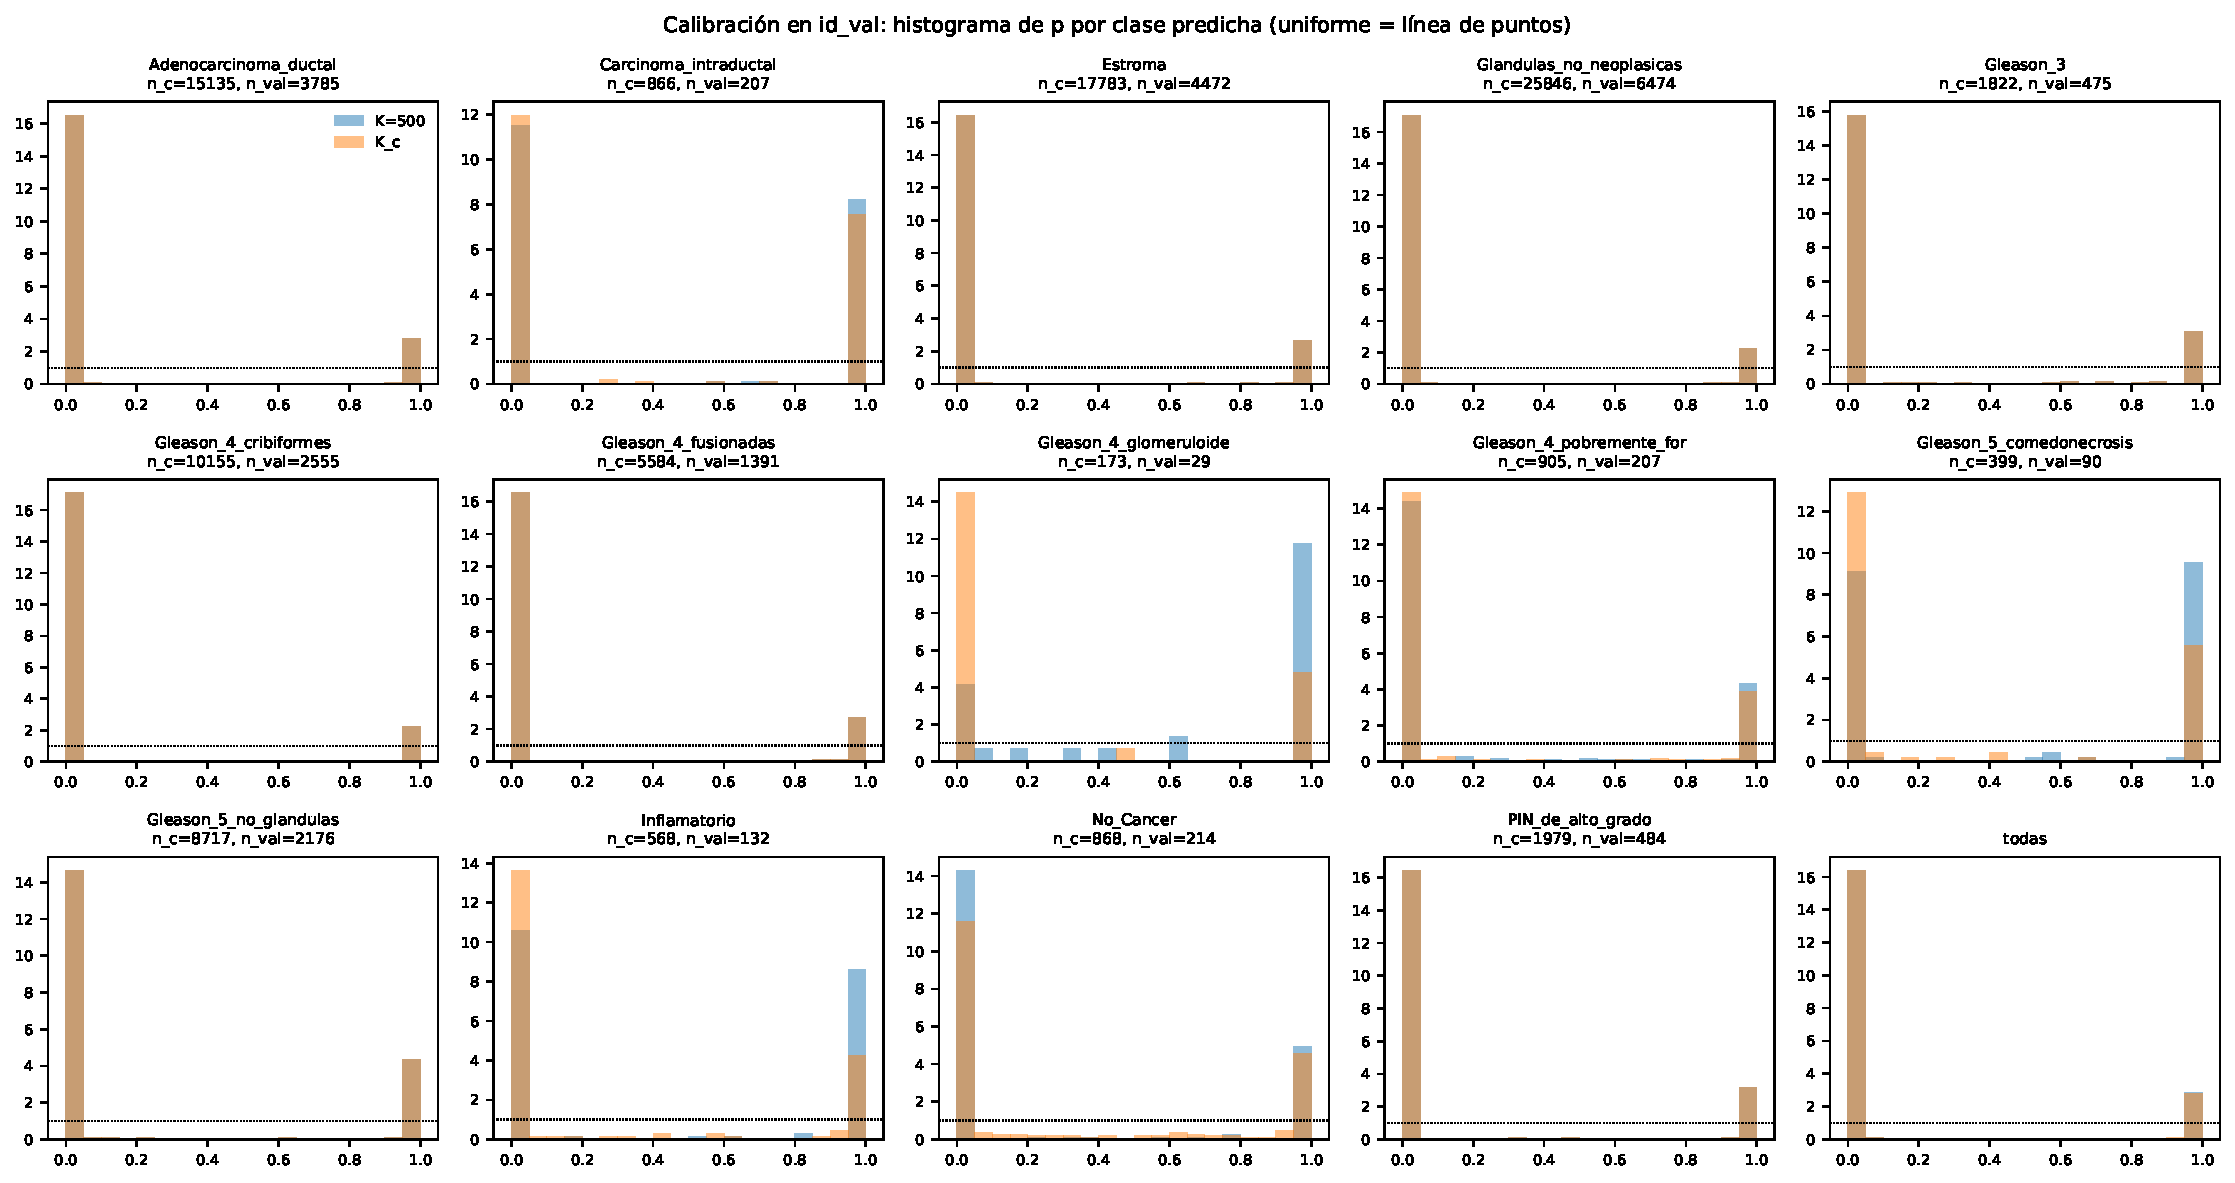
\includegraphics[width=\textwidth]{img/cap11/fig_calibracion_id_val.pdf}
  \caption{Histogramas de los $p$-valores de STOOD-X en la validación ID por clase predicha, con $K = 500$ y con $K_c$; la línea de puntos es la densidad uniforme, que se obtendría si el test estuviera calibrado. Los $p$-valores son bimodales en 0 y 1.}
  \label{fig:stoodx-calibracion}
\end{figure}

% Cifras: KS D = 0,80 frente a U(0,1); p = 0 en el 8,1 % y p = 1 en el 7,3 %. Las únicas clases
% con p menos extremo son las pequeñas (comedonecrosis, n_c = 399; glomeruloide, n_c = 173).

\section{Sensibilidad a $K$}\label{sec:stoodx-k}

En un análisis de sensibilidad sobre un subconjunto (\cref{tab:stoodx-barrido-k}), el rendimiento mejora hasta $K \approx 72$--$288$ y se degrada con $K = 500$. La degradación se concentra en las imágenes predichas en clases con pocas imágenes de entrenamiento (\clase{Gleason\_5\_comedonecrosis}, 399; \clase{Inflamatorio}, 568; \clase{No\_Cancer}, 868), donde $K$ se aproxima al tamaño de la clase y se pierde la localidad del vecindario. En particular, el 10\,\% de las imágenes de TUM + NORM se predice como \clase{Gleason\_5\_comedonecrosis}. Al excluir esas clases, la caída desaparece. Como usa datos del test ID y de los conjuntos OOD, este análisis no se ha utilizado para elegir $K$, que se elige solo con datos ID (\cref{sec:stoodx-seleccion-k}); el valor elegido, $K = 144$, está dentro del intervalo en el que el barrido obtiene los mejores resultados. Una variante que adapta $K$ al tamaño de la clase ($K_c = \min(500, \lfloor n_c/2 \rfloor)$) no mejoró los resultados.
\revisar{cambiado «que se mantiene en el valor del artículo» por la remisión a la selección de $K$ solo con datos ID}

% Generado por scripts/generar_tablas.py a partir de results_ood/stoodx_validacion/barrido_K_y_configuraciones.csv. No editar a mano.
\begin{table}
\centering
\scriptsize
\setlength{\tabcolsep}{2.5pt}
\caption{Sensibilidad de \stoodx al número de vecinos $K$ (análisis de sensibilidad; \emph{no} se usa para elegir $K$).}
\label{tab:stoodx-barrido-k}
\begin{tabular*}{\linewidth}{@{\extracolsep{\fill}}lcccccccccc}
\toprule
& \multicolumn{2}{c}{TUM+NORM} & \multicolumn{2}{c}{LYM} & \multicolumn{2}{c}{PANDA} & \multicolumn{2}{c}{DTD} & Tiempo & $p=0$ \\
\cmidrule(lr){2-3}\cmidrule(lr){4-5}\cmidrule(lr){6-7}\cmidrule(lr){8-9}
$K$ & \AUROC & \FPRn{95} & \AUROC & \FPRn{95} & \AUROC & \FPRn{95} & \AUROC & \FPRn{95} & (ms/img) & test ID \\
\midrule
9 & 0{,}933 & 0{,}132 & 0{,}936 & 0{,}218 & 0{,}897 & 0{,}326 & 0{,}937 & 0{,}132 & 0{,}7 & 0{,}0\,\% \\
18 & 0{,}962 & 0{,}067 & 0{,}955 & 0{,}212 & 0{,}917 & 0{,}270 & 0{,}966 & 0{,}067 & 0{,}5 & 0{,}0\,\% \\
36 & 0{,}976 & 0{,}042 & 0{,}963 & 0{,}179 & 0{,}917 & 0{,}289 & 0{,}978 & 0{,}042 & 0{,}6 & 0{,}0\,\% \\
72 & 0{,}985 & 0{,}030 & 0{,}968 & 0{,}165 & 0{,}922 & 0{,}272 & 0{,}986 & 0{,}030 & 0{,}8 & 0{,}0\,\% \\
144 & 0{,}988 & 0{,}030 & 0{,}962 & 0{,}161 & 0{,}924 & 0{,}248 & 0{,}988 & 0{,}031 & 1{,}3 & 0{,}0\,\% \\
288 & 0{,}988 & 0{,}040 & 0{,}944 & 0{,}235 & 0{,}926 & 0{,}236 & 0{,}988 & 0{,}038 & 4{,}6 & 0{,}0\,\% \\
500 & 0{,}952 & 0{,}342 & 0{,}890 & 0{,}554 & 0{,}877 & 0{,}462 & 0{,}986 & 0{,}040 & 14{,}4 & 9{,}1\,\% \\
\midrule
500 (87,5\,\%) & 0{,}952 & 0{,}346 & 0{,}889 & 0{,}553 & 0{,}877 & 0{,}464 & 0{,}985 & 0{,}041 & 14{,}4 & 9{,}2\,\% \\
$K_c$$^{\dagger}$ & 0{,}941 & 0{,}474 & 0{,}790 & 0{,}428 & 0{,}900 & 0{,}291 & 0{,}985 & 0{,}045 & 13{,}2 & 9{,}0\,\% \\
\bottomrule
\end{tabular*}

\smallskip
\parbox{\linewidth}{\scriptsize Subconjunto de validación: 1.000 imágenes del test ID (estratificadas por clase) y 500 de cada conjunto OOD, semilla 0. Puntuación $-z$; 100\,\% de las características salvo indicación. \AUROC: más alto es mejor; \FPRn{95}: más bajo es mejor. Tiempo por imagen: GPU (cálculo de distancias) más CPU (test de Mann-Whitney). Última columna: proporción del test ID con $p=0$ exacto (subdesbordamiento). $^{\dagger}$Variante exploratoria $K_c=\min(500,\lfloor n_c/2\rfloor)$.}
\end{table}


\begin{figure}[tbp]
  \centering
  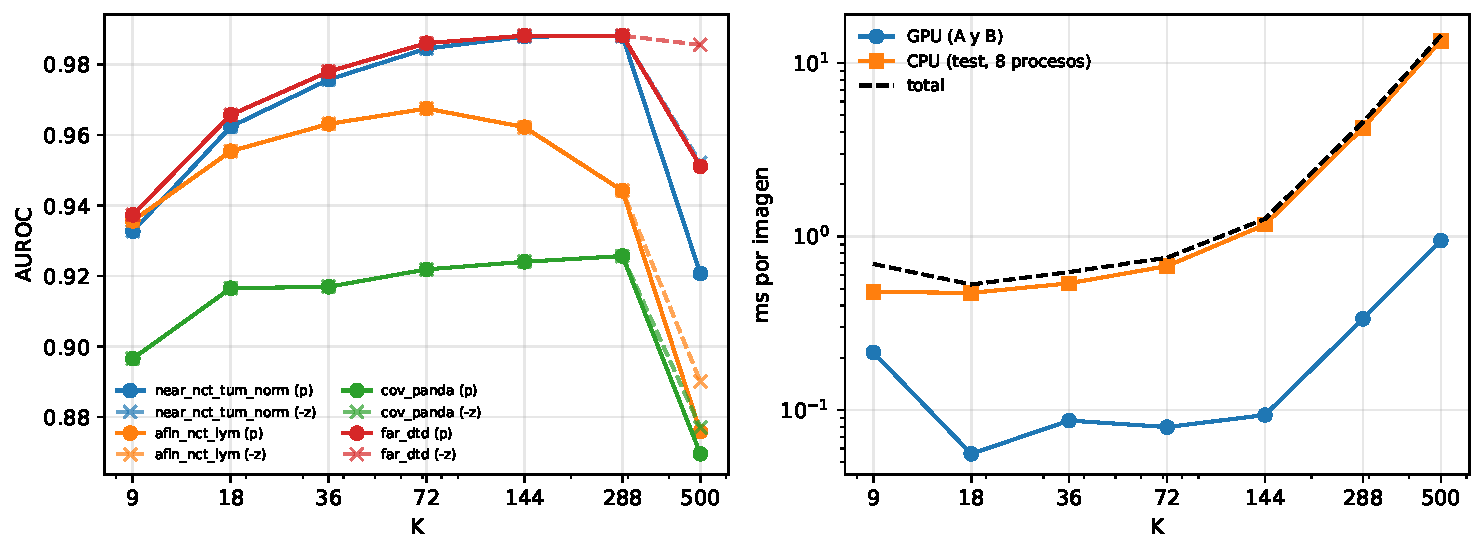
\includegraphics[width=\textwidth]{img/cap11/fig_barrido_K.pdf}
  \caption{Izquierda: AUROC con $p$ y con $-z$ frente a $K$ en TUM+NORM, LYM, PANDA y DTD. Derecha: tiempo por imagen (GPU, CPU y total) frente a $K$, en escala logarítmica. Muestra la caída con $K = 500$ y la diferencia entre $p$ y $-z$ por subdesbordamiento.}
  \label{fig:stoodx-barrido-k}
\end{figure}

% Cifras: con K = 500, p = 0 exacto en el 89 % de TUM+NORM, el 98 % de DTD y el 9 % del test ID
% (subconjunto), y p pierde hasta 0,05 de AUROC frente a -z. K_c: TUM+NORM 0,943 frente a 0,953 y
% LYM 0,799 frente a 0,903, aunque mejora PANDA (0,917 frente a 0,895).

\section{Explicaciones por ejemplos}\label{sec:stoodx-ejemplos}

Siguiendo la segunda etapa del método, la \cref{fig:stoodx-ejemplos-aceptadas} muestra imágenes representativas junto a sus cinco vecinos más cercanos de entrenamiento. Las imágenes de colon aceptadas como ID se predicen en su totalidad como \clase{Gleason\_5\_comedonecrosis}, lo que ilustra visualmente el efecto descrito.

En cada figura, la primera columna es la imagen evaluada y las cinco siguientes, sus vecinos de entrenamiento, con la clase predicha, la puntuación ($p$ y $z$) y las distancias en los títulos.

\begin{figure}[tbp]
  \centering
  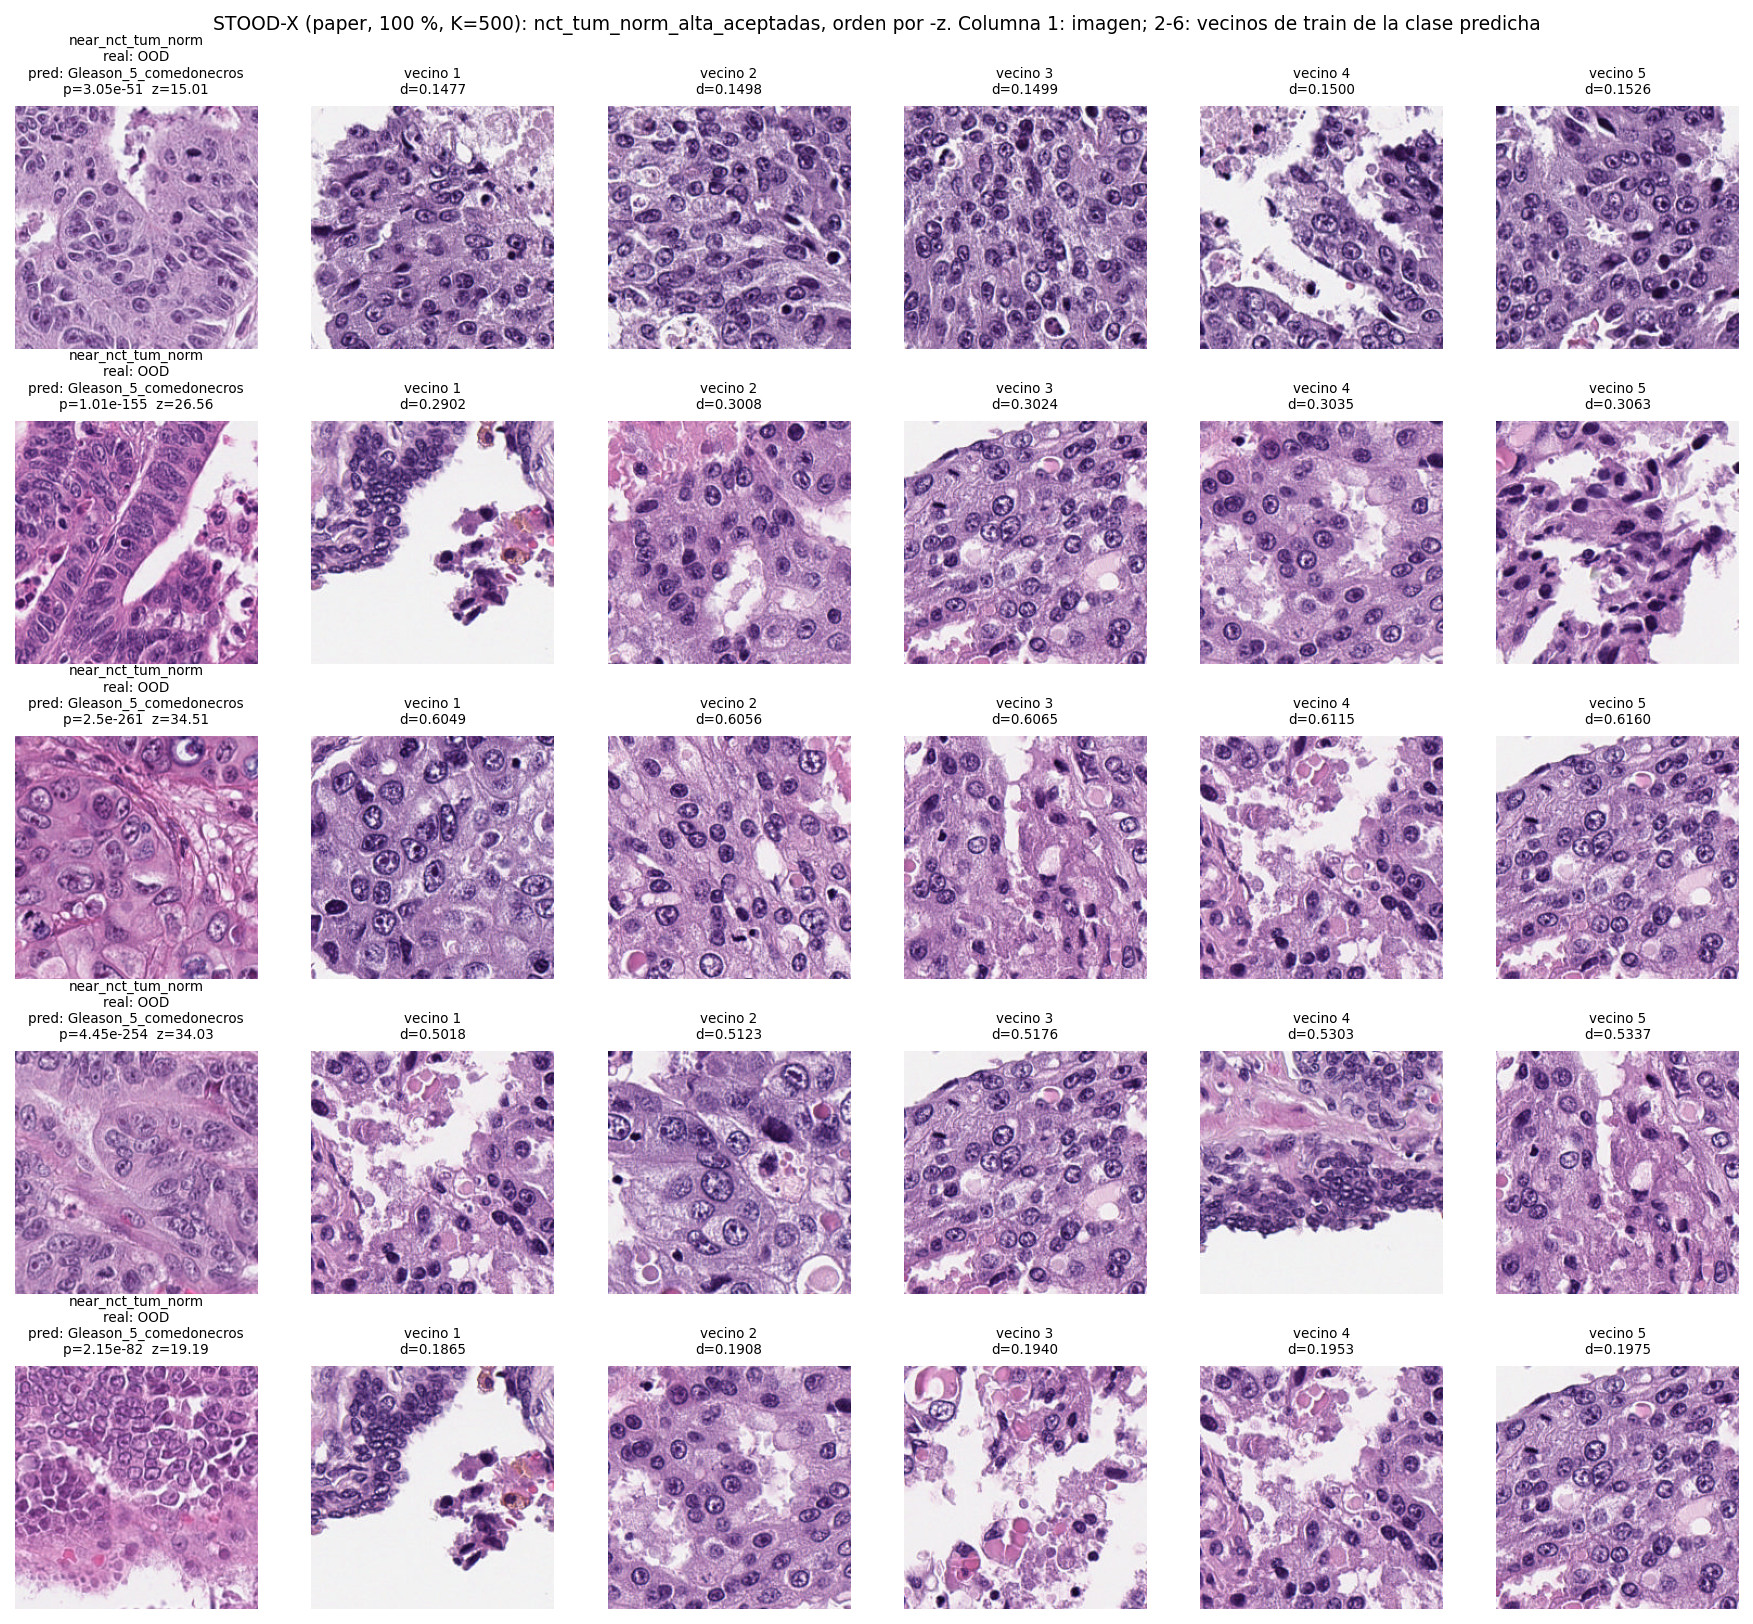
\includegraphics[width=\textwidth]{img/cap11/ejemplos_K500_nct_tum_norm_alta_aceptadas.jpg}
  \caption{STOOD-X ($K = 500$): cinco imágenes de TUM+NORM aceptadas como ID (puntuación $-z$ más alta) y sus cinco vecinos de entrenamiento de la clase predicha. Las cinco se predicen como \clase{Gleason\_5\_comedonecrosis} ($n_c = 399 < K$).}
  \label{fig:stoodx-ejemplos-aceptadas}
\end{figure}

% Cifras: las falsas alarmas ID son Adenocarcinoma ductal, Estroma y Glándulas no neoplásicas con
% z \approx 38 (separación completa).
% Resto de ejemplos (K = 500 y variante K_c) en el \cref{ap:complementario}.
\pendiente{análisis de los ejemplos del \cref{ap:complementario} (\cref{fig:stoodx-ejemplos-detectadas,fig:stoodx-ejemplos-id,fig:stoodx-ejemplos-falsas,fig:stoodx-ejemplos-lym,fig:stoodx-ejemplos-dtd}; variante $K_c$: \cref{fig:stoodx-kc-id-alta})}

\section{Discusión}\label{sec:stoodx-discusion}

% Puntos para la discusión del capítulo: competitivo en AUROC en el near-OOD y el mejor en far-OOD,
% pero con peor FPR@95 en el near-OOD, muy sensible a la resolución, saturación acotada,
% p-valores no calibrados (solo sirven para ordenar), degradación con K cercano a n_c y resultado
% negativo de K_c. Con K = 144 (elegido solo con ID): mejor AUROC en 8 de 9 conjuntos (no en LYM),
% supera a RMDS en TUM+NORM (-0,037 [-0,040; -0,035]); limitaciones: solo Swin, la clase retenida como
% pseudo-OOD, calibración no comprobada con K = 144; saturación mayor que con K = 500 (86 % de TUM+NORM) pero
% sin efecto en las conclusiones (\cref{tab:stoodx-saturacion-k144}).
\pendiente{discusión global}

\endinput
